\documentclass[../main]{subfiles}
\begin{document}
    \setcounter{secnumdepth}{2}
    \chapter{序論}
        \section{背景}
        近年,商業施設での清掃作業や屋外での宅配など,屋内外を問わず多くの場所で自律移動ロボットが活用されている.
        それらのロボットを安全かつ正確に運用するためには,自己位置推定をはじめとする様々な機能を持たせる必要がある.
        現在,商業施設などで用いられている自律移動ロボットは,あらかじめセンサにより取得した環境の詳細なデータを持つメトリックマップと呼ばれる
        地図を用いて,自己位置推定を行なっている.しかし,詳細な地図を用いた自己位置推定は,事前に取得した地図に存在しないものが環境中に置かれると
        自己位置推定に致命的な支障をきたすという問題がある.
        
        
        一方,人はそのような詳細な地図がなくても,「次の交差点で右」のような言葉の情報に基づき目的地まで移動することができる.
        そこで,そのような人の移動する能力をロボットの自律移動に応用する手法が研究されている.
        例えば,島田らは人の道案内に注目し,人の道案内のようにロボットを目的地まで移動させるナビゲーションの手法を提案した\cite{shimada_paper1}\cite{shimada_paper2}.
        この研究では,人が道案内により移動する際,歩行者の向きや三叉路や突き当たりなどの通路の特徴(形状)を重視しているということをアンケートにより収集し,
        ナビゲーションに用いるトポロジカルマップと呼ばれる地図と,シナリオと呼ばれる道案内を文章で表現したものの形式を決め,
        実ロボットでの実験により提案したナビゲーション手法の有効性を検証した.
        検証の結果,通路の特徴の分類が正しく行われた場合は提案したナビゲーション手法により目的地に到達できるが,
        通路の特徴の分類に失敗した場合はロボットが経路から外れ,ナビゲーションに失敗してしまうということが報告されている.
        提案手法の通路の分類はChenらが提案するLiDARを用いた通路検出手法(Toe-Finding Algolithm)\cite{toe-finding_paper}を参考にしており,
        LiDARの周囲に壁などの遮蔽物がなく,開けている方向があればその方向に通路があると検出する.
        先行研究の通路分類に失敗した原因は,開いているドアや隙間がある方向に通路があbv誤検出したからであると述べられている.
        そこで,通路の特徴分類にカメラ画像を用いることで通路の誤検出を解消できるのではないかと考えた.

        \newpage

        \section{目的}
        本研究は,全天球カメラ画像に基づく通路の分類手法を提案する.
        具体的には,全天球カメラで水平360度の画像を取得し,取得した画像からYOLOの学習器を用いて\fref{figure::image_exp}に示すように通路やドアなどの物体を検出する.
        また,検出した通路とその方向からどの通路の特徴に相当するかを分類する手法である.
        全天球カメラを取り付けたロボットを実験環境の24箇所の通路に移動させ,提案した手法により通路の分類が行えるかどうかを検証する.
        
        また,本研究では全天球カメラの標準的なフォーマットである正距円筒図法という形式で画像を扱う.
        
        \begin{figure}[H]
            \centering
            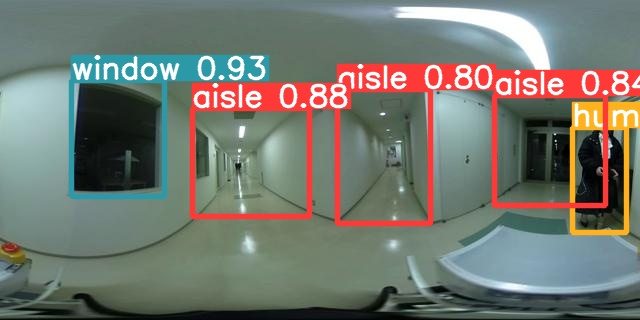
\includegraphics[width=10cm]{../images/yolo_aisle.jpg}
            \caption{Detecting an object using YOLO}
            \label{figure::image_exp}
        \end{figure}
        
        \newpage

        \section{関連研究}
        

        \section{本論文の構成}
        本論文ではまず,第1章で研究背景,目的,関連研究について述べた.第2章では,本研究で用いる要素技術について述べる.また,第3章では提案した手法について述べ,
        第4章では提案した手法の有効性の検証を行う.また,第5章では4章で行なった実験の結果をまとめ,考察を行う.最後に,第6章で本研究のまとめを行う.
\end{document}